%; whizzy paragraph -pdf xpdf -latex ./whizzypdfptex.sh
%; whizzy-paragraph "^\\\\begin{frame}\\|\\\\emtext"
% latex beamer presentation.
% platex, latex-beamer $B$G%3%s%Q%$%k$9$k$3$H$rA[Dj!#(B 

%     Tokyo Debian Meeting resources
%     Copyright (C) 2012 Junichi Uekawa

%     This program is free software; you can redistribute it and/or modify
%     it under the terms of the GNU General Public License as published by
%     the Free Software Foundation; either version 2 of the License, or
%     (at your option) any later version.

%     This program is distributed in the hope that it will be useful,
%     but WITHOUT ANY WARRANTY; without even the implied warreanty of
%     MERCHANTABILITY or FITNESS FOR A PARTICULAR PURPOSE.  See the
%     GNU General Public License for more details.

%     You should have received a copy of the GNU General Public License
%     along with this program; if not, write to the Free Software
%     Foundation, Inc., 51 Franklin St, Fifth Floor, Boston, MA  02110-1301 USA

\documentclass[cjk,dvipdfm,12pt]{beamer}
\usetheme{Tokyo}
\usepackage{monthlypresentation}

%  preview (shell-command (concat "evince " (replace-regexp-in-string "tex$" "pdf"(buffer-file-name)) "&")) 
%  presentation (shell-command (concat "xpdf -fullscreen " (replace-regexp-in-string "tex$" "pdf"(buffer-file-name)) "&"))
%  presentation (shell-command (concat "evince " (replace-regexp-in-string "tex$" "pdf"(buffer-file-name)) "&"))

%http://www.naney.org/diki/dk/hyperref.html
%$BF|K\8l(BEUC$B7O4D6-$N;~(B
\AtBeginDvi{\special{pdf:tounicode EUC-UCS2}}
%$B%7%U%H(BJIS$B7O4D6-$N;~(B
%\AtBeginDvi{\special{pdf:tounicode 90ms-RKSJ-UCS2}}

\title{$BEl5~%(%j%"(BDebian$BJY6/2q(B}
\subtitle{$BBh(B96$B2s(B 2013$BG/(B1$B7nEY(B}
\author{$B>e@n=c0l(B\\dancer@debian.org}
\date{2013$BG/(B1$B7n(B19$BF|(B}
\logo{
\includegraphics[width=8cm]{image200607/openlogo-light.eps}}

\begin{document}

\frame{\titlepage{}}

\begin{frame}{$B@_1D=`Hw$K$46(NO$/$@$5$$!#(B}
$B2q>l@_1D$h$m$7$/$*$M$,$$$7$^$9!#(B
\end{frame}

\begin{frame}{Agenda}
\begin{minipage}[t]{0.45\hsize}
  \begin{itemize}
  \item $BCm0U;v9`(B
	\begin{itemize}
	 \item $BIt20FbIt0J30$N<L??;#1F(B
	\end{itemize}
   \item $B:G6a$"$C$?(BDebian$B4XO"$N%$%Y%s%HJs9p(B
	\begin{itemize}
        \item $BBh(B95$B2s(B $BEl5~%(%j%"(BDebian$BJY6/2q(B
	\end{itemize}
   \item $B;vA02]Bj>R2p(B
 \end{itemize}
\end{minipage} 
\begin{minipage}[t]{0.45\hsize}
 \begin{itemize}
  \item Debian$BJY6/2q%"%s%1!<%H(B
  \item 2013-2015$BG/$rLQA[$9$k(B
  \item gdb python$B3HD%$=$N(B1
  \item $B7n4)(BDebhelper
 \end{itemize}
\end{minipage}
\end{frame}


\section{$B%$%Y%s%HJs9p(B}
\emtext{$B%$%Y%s%HJs9p(B}
\begin{frame}{$BBh(B95$B2s(B $BEl5~%(%j%"(BDebian$BJY6/2q(B}
\begin{itemize}
\item $B3+:E>l=j$O(B $B$"$s$5$s$V$k2.7&$G$7$?!#(B
\item im-config$B$N>R2p(B
\item 2012$BG/$N(BDebian$BJY6/2q$N?6$jJV$j(B
\item DFSG$B$H(B2012$BG/2~@5Cx:n8"K!$K$D$$$F$NH/I=(B
\end{itemize}
$B$,$"$j$^$7$?!#(B
\end{frame}

\section{DWN quiz}
\emtext{DWN quiz}
\begin{frame}{Debian $B>o<1%/%$%:(B}

Debian $B$N>o<1!"$b$A$m$sCN$C$F$^$9$h$M(B?
$BCN$i$J$$$J$s$FCQ$:$+$7$/$F!"CN$i$J$$$H$O8@$($J$$$"$s$J$3$H$d$3$s$J$3$H!"(B
$B$_$s$J$G3NG'$7$F$_$^$7$g$&!#(B

$B:#2s$N=PBjHO0O$O(B\url{debian-devel-announce@lists.debian.org},
\url{debian-devel@lists.debian.org} $B$KEj9F$5$l$?(B
$BFbMF$H(BDebian Project News$B$J$I$+$i$G$9!#(B

\end{frame}

\subsection{$BLdBj(B}
%; whizzy-master ../debianmeetingresume201211.tex
% $B0J>e$N@_Dj$r$7$F$$$k$?$a!"$3$N%U%!%$%k$G(B M-x whizzytex $B$9$k$H!"(Bwhizzytex$B$,MxMQ$G$-$^$9!#(B
%

\santaku
{wiki.debian.org$B$G;H$o$l$F$$$?(Bwiki$B%7%9%F%`$N%=%U%H%&%'%"$NL>A0$O!)(B}
{pukiwiki}
{mine}
{moin}
{C}
{$B@?$K0d48$J$,$i!"(Bwiki.debian.org$B$,$3$NA0%/%i%C%/$5$l$?$h$&$G$9!#(B
$BB>$GF1$8EPO?%a!<%k%"%I%l%9$H%Q%9%o!<%I$NAH$r;H$C$F$$$k?M$O!"(B
$B$9$0$K%Q%9%o!<%I$rJQ$($?J}$,$h$$$G$7$g$&!#(B}

\santaku
{$B5nG/$NG/Kv$N(Bpopcon$BD4::$G(BNo.1$B$K51$$$?%W%i%C%H%U%)!<%`$O!)(B}
{$BEvA3(Barmel$B$@$m!)(B}
{i386}
{amd64}
{C}
{\url{http://popcon.debian.org/}$B$N%H%C%W%Z!<%8$K7k2L$N%0%i%U$,$"$j$^$9!#(B
 $B:#$^$G(BNo.1$B$r7h$a$F$$$?(Bi386$B$rG/Kv$G(Bamd64$B$,H4$-5n$C$?$h$&$G$9!#(B}

\santaku
{1$B7nF,$N(BDPN$B$GJs9p$N$"$C$?!"(Bwheezy$B$K;D$C$F$$$k(BRC$B%P%0$N?t$O(B1$B7n(B5$BF|;~E@$G$"$H2?8D!)(B}
{$B$"$H(B321$B8D(B}
{$B$"$H(B171$B8D(B}
{$B$"$H(B17$B8D(B}
{B}
{$B4JC1$KD>$;$k(B/$BB><#$l$P>!<j$K<#$j$=$&$b$N$r4^$s$G(B171$B8D!#<j$,$+$+$j$=$&$J$N$O(B
$B$@$$$?$$(B116$B8D$@$=$&$G$9!#(B}

\santaku
{$B:#G/(Bamazon$B$+$i(BDebian Project$B$X$$$/$i$+$N(BAWS$B$NMxMQ7t$r%9%]%s%5!<$7$F$b$i$C$?$=$&$J$N$G$9$,!"6b3[$K$9$k$H$*$$$/$i!)(B}
{8000USD}
{800USD}
{80000USD}
{A}
{$BF|K\1_$K$9$k$HLs(B72$BK|1_J,$NMxMQ7t!#(BQA$B$K$O==J,$H$N$3$H$G$7$?!#(B}












\section{$B;vA02]Bj(B}
\emtext{$B;vA02]Bj(B}
{\footnotesize
 %; whizzy-master ../debianmeetingresume201301.tex
% $B0J>e$N@_Dj$r$7$F$$$k$?$a!"$3$N%U%!%$%k$G(B M-x whizzytex $B$9$k$H!"(B
% whizzytex$B$,MxMQ$G$-$^$9(B

\begin{prework}{$B>e@n=c0l(B}

\preworksection{2013$BG/$NJY6/2q$GH/I=$7$?$$FbMF$r65$($F$/$@$5$$(B}
\preworksection{2015$BG/$G$O(BDebian$B$,$I$&$J$C$F$$$k$+$rBgC@$KM=A[$7$F$/$@$5$$(B}


\end{prework}

}

\section{Debian$BJY6/2qM=Ls%7%9%F%`%"%s%1!<%H=87W(B}
\emtext{Debian$BJY6/2qM=Ls%7%9%F%`%"%s%1!<%H=87W(B}
\section{2015$BG/$rLQA[$9$k(B}
\emtext{2015$BG/$rLQA[$9$k(B}
\begin{frame}{2015$BG/$rLQA[$9$k(B}
 
 { \tiny
\begin{tabular}[t]{|p{8.5em}|p{12em}|p{8em}|p{6em}|p{8em}|}
 \hline
 2011 &2012 & 2013 & 2014 & 2015 \\
 \hline

 %2011

 $B%G%9%/%H%C%W%Q%=%3%s=*N;$ND,N.!#(B

 cpu$B%3%"C1BN$G$O9bB.2=$7$J$$$h$&$K!#(B

 webos$B=*N;$N$*CN$i$;!#(B

 adobe flash$BI|3h$N$*CN$i$;(B($B%-%?(B), silverlight$B=*N;$N$*CN$i$;(B($BBfOQ$r=|$/(B)($BB3$$$F$k(B?)

 squeeze$B%j%j!<%9(B($B$*$a$G$H$&(B)

 ipv4$B3d$jEv$F$N=*N;$N$*CN$i$;(B($B%-%?(B)

 $BCO>eGH%G%8%?%k0\9T1dD9!#(B

 btrfs$B$^$@4hD%$k(B(fedora$B25(B)

 java$B=*N;(B(sun java$B=*N;(B)

 open office$B$,(Boracle office$B$K(B($B%J%$(B)

 &
 %2012

 $B%N!<%H%Q%=%3%s$h$j%?%V%l%C%H$N$[$&$,Gd$l$F$$$k!#(B
 $B%N!<%H%Q%=%3%s$G$O(Bmacbookair$B$,>o<1$K!#(B

 $B%N!<%H%Q%=%3%s$G(Bintel$B$8$c$J$$$b$N(B(mips/arm)$B$,<gN.$K$O$^$@$J$i$:!#%?%V%l%C(B
 $B%H$N$[$&$,<gN.!#(B

 $B%G%9%/%H%C%W(B:$B%2!<%`0J30$NMQES$G$O=*N;$7$F$$$k!#(B

 $B%5!<%P(B:$B$[$H$s$I(Bvps$B$+!#(B

 $B7HBSEEOC(B:
 $B%,%i%Q%4%9$N=*_a!#F|K\$G$N7HBSEEOCHNGd$G$b%9%^!<%H%U%)%s$,#5#0!s$rD6$($k$h$&$K!#(B
 lte$B$,<gN.$K$J$C$F$$$J$$!#(B
 softbank$B$NFsG/7@Ls$O$^$@B3$$$F$$$k!#(Bsim free$B$X$NF;$O9L$5$l$?$,$"$?$jA0$K$J$i$J$+$C$?!#(B

 btrfs$B$O$^$@@8$-;D$C$F$$$k!#(B

 mysql$B$+$i(Bmariadb$B$,GI@8!#(B

 & 
 % 2013
 \vspace{0.5\vsize}
 .
 & 
 % 2014
 & 
 % 2015

 \\

 \hline
 \end{tabular}

 }
\end{frame}

\begin{frame}{2013$BG/$N7W2hDs0F(B}

 $B<j85$N;qNA$K=q$-=P$7$F$_$F$/$@$5$$(B 
\end{frame}

\begin{frame}{2013$BG/$N7W2h(B}

{
\begin{enumerate}
 \item 2013$BG/$N7W2hN)0F(B
 \item \underline{(\hspace{8cm})}
 \item \underline{(\hspace{8cm})}
 \item \underline{(\hspace{8cm})}
 \item \underline{(\hspace{8cm})}
 \item \underline{(\hspace{8cm})}
 \item \underline{(\hspace{8cm})}
 \item \underline{(\hspace{8cm})}
 \item \underline{(\hspace{8cm})}
 \item \underline{(\hspace{8cm})}
 \item \underline{(\hspace{8cm})}
 \item $B0lG/4V$NH?>J(B
\end{enumerate}
}
\end{frame}

\section{gdb python$B3HD%$=$N(B1}
\emtext{gdb python$B3HD%$=$N(B1}
\begin{frame}{$B%G%P%C%,$N;H$$F;(B}
\Large
\begin{itemize}
 \item $B%G%P%C%0$N$*6!$K(B
 \item $B%j%P!<%9%(%s%8%K%"%j%s%0$N$*6!$K(B
\end{itemize}
\end{frame}

\begin{frame}{$B;29M!'(BOSS$B$N%j%P!<%9%(%s%8%K%"%j%s%0(B}

OSS$B$r%j%P!<%9%(%s%8%K%"%j%s%0$7$?$/$J$k>u67!'(B

\begin{itemize}
 \item $B$H$K$+$/Cj>]2=$r;H$$$3$J$7$F$k%3!<%I(B
 \item $B%G!<%?%I%j%V%s$J%3!<%I(B
 \item $B$=$b$=$b26$NM}2r$r1[$($?%3!<%I(B
\end{itemize}

$B$H@o$&;~!#(B

\center{\Large ...$B%=!<%9%3!<%IFI$s$@$@$1$G$OF0:n$,$o$+$i$s(B... }\\

 $B$G!"%G%P%C%,$G<B9T$7$FF0:n$rDI$$$+$1$k$H!"$$$m$$$m$JH/8+$,$"$C$?$j!"F0:n$,NI$/$o$+$C$?$j!"%"!<%-%F%/%A%c$,8+$($?$j$9$k!#(B
\end{frame}

\begin{frame}{gdb}

\Large
\begin{itemize}
 \item  gdb$B$H$O(B \\
$BI}9-$$%W%i%C%H%U%)!<%`$GMxMQ$G$-!"B??t$N%P%$%J%j7A<0$KBP1~$G$-!"AH$_9~$_MQES$K%j%b!<%H%G%P%C%0$^$G=PMh$k!"Hs>o$K6/NO$J%G%P%C%,!#(B
\end{itemize}

\end{frame}

\begin{frame}{gdb+python}
\Large
\begin{itemize}
\item gdb v7.0$B$+$i(Bgdb$B$K(Bpython$B$,9gBN!*(B
\item Debian sid$B:-Jq$N(Bgdb$B$b(Bpython$B$,M-8z(B!
\end{itemize}

\center{\Large $B6/NO$J%G%P%C%,$,$5$i$K6/NO$K(B!\\
gdb$B$b$3$l$G(Bbattelies included!}

\end{frame}

\begin{frame}{Debian sid$B$N(Bgdb$B$N(Bpython$B6q9g(B}

\begin{table}[ht]
\begin{center}
\small
\begin{tabular}{|l|l|l|}
\hline
$B9`HV(B & $B9`L\(B & $BCM(B \\
\hline
1 & gdb$B%P!<%8%g%s(B & 7.4.1 \\
2 & python$B%P!<%8%g%s(B & 2.7.3 \\
3 & python$B%5!<%A%Q%9(B & /usr/share/gdb/python,\\
 & &/usr/lib/python2.7$B0J2<(B \\
\hline
\end{tabular}
\end{center}
\end{table}

\end{frame}

\begin{frame}{$B$A$H:$$k;v(B}

\Large

 $B$H$K$+$/!"J88%$,>/$J$$(B!

\begin{itemize}
\item info gdb $B"*(BExtending GDB$B"*(Bpython$B$N9`L\$+!"(B
\item \small \url{http://sourceware.org/gdb/wiki/PythonGdbTutorial}
\end{itemize}

$B$0$i$$!#(B
\center{$BB>$K$"$C$?$i65$($F!<$C(B}

\end{frame}

\begin{frame}{$BJdB-!'$5$i$K:$$C$?;v(B}

\Large
\center{$B!V$7$^$C$?!"26$O(Bpython$B$N=q$-J}$bCN$i$J$+$C$?$J!#$=$&$$$($P!#!W(B}\\

($BB(@J$G!"J8K!$b3P$($kI,MW$,$,$,$,(B...)

\end{frame}

\begin{frame}[containsverbatim]{$B$H$j$"$($:F0$+$7$F$_$k(B}

$B$H$j$"$($:!"F0$+$7$F$_$k!#(B
(gdb)$B$O(Bgdb$B$N%W%m%s%W%H$G$9!#(B

\begin{commandline}
$gdb
(gdb) python print "hello world"
hello world
(gdb) python a=[1,2,3,4]
(gdb) python print a
[1, 2, 3, 4]
(gdb) python a.append(5)
(gdb) python print a
[1, 2, 3, 4, 5]
(gdb) python
>import sys
>print sys.path
>print sys.version_info
>$B$3$3$G(BCtrl+d
['/usr/share/gdb/python', '/usr/lib/python2.7',
  '/usr/lib/python2.7/plat-linux2', ...$BCfN,(B...
\end{commandline}
% $

\end{frame}

\begin{frame}{gdb+python$B9=B$(B}

$B%P%C%/%0%i%&%s%I$G(Bpython$BF0$+$7$F$k$s$@$m$&$H;W$C$?$iBg4V0c$$!#(B
$B<B:]$K$O(Bgdb$B$K(Bpython$B=hM}7O$r7k9g$7$F$?!#(B

\begin{figure}[h]
\begin{center}
 \includegraphics[width=0.8\hsize]{image201301/gdb-python/gdb-python-internal-schema.eps}
\end{center}

\end{figure}

\end{frame}

\begin{frame}[containsverbatim]{module gdb$B$NDj5A$O$I$3(B}

python$B$G(Bmodule$B$NDj5A$rCN$k$K$O!"(Bpydoc$B$,$"$k!#$G$b!"(B
gdb$B$NCf$K<BAu$5$l$?(Bmodule gdb$B$NDj5A$rFI$`$K$O(B...

\center{\Large python$B$N(Bhelp()$B4X?t$r8F$Y$P$$$$(B}

\begin{commandline}
(gdb) python help(gdb)
Help on package gdb:

NAME
    gdb

FILE
    (built-in)

PACKAGE CONTENTS
    command (package)
    printing
...$BCfN,(B...
\end{commandline}

\end{frame}

\begin{frame}{module gdb$B$N(Bclass$B?^$,8+$?$$(B}
\Large

$B@hDx$N(Bmodule gdb$B$NDj5A$+$i!"COF;$K(Bclass$B?^$r5/$3$7$F$_$?!#(B

$B;2>H!'Bh(B96$B2sEl5~%(%j%"(BDebian$BJY6/2q;qNA(B7.6$B>O$N?^;2>H!#(B

\end{frame}

\begin{frame}[containsverbatim]{$B4pK\E*;H$$J}!'(Bgdb$B%3%^%s%I$rA}$d$9(B($B$=$N(B1)}

gdb$B$K?75,$N%3%^%s%I$rA}$d$7!"(Bpython$B$H7k9g$9$k$K$O(Bgdb.Command$B%/%i%9(B
$B$r7Q>5$7$?%*%V%8%'%/%H$r@8@.$7$FA}$d$9!#(Bgdb$BB&$KA}$d$9%3%^%s%IL>$O(B
gdb.Command$B%*%V%8%'%/%H$N%3%s%9%H%i%/%?7PM3$GEPO?$9$k!#(B

hello.py$B$NCf?H!'(B
\begin{commandline}
import gdb                      
class HelloWorld (gdb.Command): 
  """ Greet the whole world """ 
  def __init__ (self):
     super(HelloWorld, self).__init__ ("hello-world",
$B!!!!!!!!!!!!!!!!!!!!!!!!!!!!!!!!!!(Bgdb.COMMAND_OBSCURE)

  def invoke (self,arg, from_tty): 
     print "Hello, World! arg=["+str(arg)+"]"

HelloWorld()$B!!(B
\end{commandline}

\end{frame}

\begin{frame}[containsverbatim]{$B4pK\E*;H$$J}!'(Bgdb$B%3%^%s%I$rA}$d$9(B($B$=$N(B2)}

$B<B9T$7$F$_$?!#(B

\begin{commandline}
(gdb) source hello.py
(gdb) hello-[$B$3$3$G(BTAB$B$r2!$9$HJd40$5$l$k(B]
(gdb) hello-world foo,bar,com
Hello, World! arg=[foo,bar,com]
(gdb) help obscure
Obscure features.

List of commands:

...$BCfN,(B...
hello-world --  Greet the whole world 
...$BCfN,(B...
\end{commandline}

\end{frame}

\begin{frame}[containsverbatim]{$B:n$C$?%9%/%j%W%H$N<+F0FI$_9~$_(B}

$B$$$D$b$$$D$b(B''source $B%9%/%j%W%HL>(B''$B$OLLE]$J$N$G!"<+F0$GFI$_9~$^$;$?$$;~$O!'(B

\begin{itemize}
\item \verb!$(HOME)/.gdbinit!$B$GFI$^$;$k(B
\item $B%P%$%J%jB&(B\verb!.gdb_gdb_scripts!$B%;%/%7%g%s$KKd$a9~$`(B
\item ``$B%P%$%J%jL>(B''-gdb.py$B$H$$$&L>A0$G%9%/%j%W%H$rMQ0U$9$k(B
\end{itemize}

$B$NJ}K!$,$"$j$^$9!#(B

\end{frame}

\begin{frame}[containsverbatim]{.gdbinit$B$GFI$^$;$k(B}

$B0J2<$N%U%!%$%k$r(BHOME$B%G%#%l%/%H%jG[2<$KMQ0U!'(B
\begin{commandline}
----${HOME}/.gdbinit$B$3$3$+$i(B-----
source /home/foo/bar/my-gdb-func.py
----${HOME}/.gdbinit$B$3$3$^$G(B-----
\end{commandline}
\end{frame}

\begin{frame}[containsverbatim]{.gdb\_gdb\_scripts$B$GFI$^$;$k(B}

$B0J2<$N(Basm$BL?Na$rBG$A9~$s$G$*$/!#(B
\begin{commandline}
asm(
".pushsection \".debug_gdb_scripts\",\"MS\",@progbits,1\n"
".byte 1\n"
".asciz \"hello.py\"\n"
".popsection \n"
);
\end{commandline}

\center{\Large $B$A$H@H<e@-$N9a$j$,(B...}

\end{frame}

\begin{frame}[containsverbatim]{``$B%P%$%J%jL>(B''-gdb.py$B$GFI$^$;$k(B}

\begin{commandline}
$ ls 
hello hello-gdb.py hello.c
\end{commandline}
%$

gdb hello$B$H$9$k$H!"(Bhello-gdb.py$B$,<+F0$GFI$_9~$^$l$k!#(B

\end{frame}

\begin{frame}[containsverbatim]{$B4pK\E*;H$$J}!'(Bbreakpoint$B$rA`$k(B}

gdb.Breakpoint $B%/%i%9$r7Q>5$7$?%*%V%8%'%H$rMQ0U$9$k$H!"(B
$B;XDj$7$?(Bbreakpoint$B$GFCDj$N=hM}$r$5$;$k;v$,2DG=!#(B

main$B$G(Bbreak$B$7$F(Bhi!$B$HI=<($9$kNc!'(B
\begin{commandline}
class _ExampleBreakpoint(gdb.Breakpoint):
   def __init__(self, spec):
       super(_ExampleBreakpoint, 
            self).__init__(spec,gdb.BP_BREAKPOINT,
                          internal = False)
   def stop(self):
        print "hi!"

_ExampleBreakpoint("main")
\end{commandline}

gdb.BP\_BREAKPOINT$B$r;XDj$9$k$H!"(Bbreakpoint$B$K$J$j!"(B
gdb.BP\_WATCHPOINT$B$r;XDj$9$k$H!"(Bwatchpoint$B$H$J$k!#(B
\end{frame}

\begin{frame}[containsverbatim]{$B4pK\E*;H$$J}!'(Bfinish$B$rA`$k(B}

gdb.FinishBreakpoint $B%/%i%9$r7Q>5$7$?%*%V%8%'%H$rMQ0U$9$k$H!"(B
$B8=:_$N%9%?%C%/%U%l!<%`$+$iHt$S=P$h$&$H$9$k$H(Bbreak$B$9$k!#(B

$B%9%?%C%/%U%l!<%`$+$i=P$k$H(Bhi!$B$HI=<($9$kNc!'(B
\begin{commandline}
class _ExFinishBreakpoint(gdb.FinishBreakpoint):
   def __init__(self):
        super(_ ExFinishBreakpoint, 
              self).__init__(internal=False)
   def stop(self):
        print "hi!"

   def out_of_scope(self):
        print "hi!"
\end{commandline}

stop()$B$O!"(Breturn$B$K$h$j%9%?%C%/%U%l!<%`$+$i=P$k>l9g!"(Bout\_of\_scope()$B$O(Blongjump$B$H$+(B
$B$G0l5!$KHt$S=P$9>l9g$K(Bbreak$B$9$k!#(B

\end{frame}

\begin{frame}[containsverbatim]{$B4pK\E*;H$$J}!'%3%^%s%I$N7k2L$rF@$k(B}

gdb$B$N%3%^%s%I$N<B9T7k2L$rF@$k;v$,$G$-$k$HJXMx$J>l9g$,$"$j$^$9!#(B

\begin{commandline}
result=gdb.execute('info break',False,True)
\end{commandline}

result$B$K(Bgdb$B$N%3%^%s%I(B''info break''$B$N7k2L$,J8;zNs%/%i%9$G3JG<$5$l$^$9!#(B

\end{frame}

\begin{frame}{$B0J>e$r3hMQ$7$F$_$?Nc(B}

 $B2r@OMQES$G!"%W%m%0%i%`$N%3!<%k%D%j!<$r<h$C$F$_$?$+$C$?!#(B

 $B6qBNE*$J%9%/%j%W%H$N%=!<%9$H;H$$J}$O!"(B\\
$BBh(B96$B2sEl5~%(%j%"(BDebian$BJY6/2q;qNA(B7.9$B>O;2>H!#(B

\end{frame}

\begin{frame}{calltracer.py$BF0:n@bL@(B}

\begin{description}
\item [Step 1.] rbreak$B$r<B9T$7$F!"%G%P%C%0>pJs$K$"$kA44X?t$K0lC6(Bbreakpoint$B$r;E3]$1$k(B
\item [Step 2.] info break$B$N7k2L$r%Q!<%9$7$F!"4X?t$N%"%I%l%9$H!"L>A0$NN>J}$rF@$k!#(B
\item [Step 3.] $B%+%9%?%^%$%:$7$?(Bbreakpoint$B$HF~$lBX$($k!#(B
\item [Step 4.] break$B$7$?$i!"%9%?%C%/DI@WJQ?t(B(self.stack)$B$r(B+1$B$7$F4X?tL>$rI=<(!#F1;~$K%+%9%?%^%$%:$7$?(Bfinish$B$r;E3]$1$k!#(B
\item [Step 5.] finish$B$G(Bbreak$B$7$?$i!"4X?tL>$rI=<($7$F%9%?%C%/DI@WJQ?t$r(B-1$B$9$k!#(B
\item [Step 6.] Step 4.$B!A(BStep 5.$B$r7+$jJV$9!#(B
\end{description}

\end{frame}

\begin{frame}{$B=*$o$j$K(B}

\center{\Large python$B$N$*$+$2$G!"(B\\$B$J$s$+$b$&L4$R$m$,$j$s$0(B\\
$B$^$@$^$@5!G=K~:\$J$N$G!"(B\\$B<!2s$bH/I=B3$1$k$h$I$3$^$G$b(B!}

\end{frame}

\section{$B7n4)(BDebhelper}
\emtext{$B7n4)(BDebhelper}


\section{$B:#8e$N%$%Y%s%H(B}
\emtext{$B:#8e$N%$%Y%s%H(B}
\begin{frame}{$B:#8e$N%$%Y%s%H(B}
\begin{itemize}
 \item 2013$BG/(B2$B7n(B OSC Tokyo
 \item 2013$BG/(B3$B7n(B Debian$BJY6/2q(B
\end{itemize}
\end{frame}

\section{$B:#F|$N1c2q>l=j(B}
\emtext{$B:#F|$N1c2q>l=j(B}
\begin{frame}{$B:#F|$N1c2q>l=j(B}
$BL$Dj(B
\end{frame}

\end{document}

;;; Local Variables: ***
;;; outline-regexp: "\\([ 	]*\\\\\\(documentstyle\\|documentclass\\|emtext\\|section\\|begin{frame}\\)\\*?[ 	]*[[{]\\|[]+\\)" ***
;;; End: ***
